\chapter{Security Recommendations}

This section will combine the results in the last section to provide security
recommendations for Verified Boot.
While no security holes were found in Verified Boot, specific additions to the
Vboot process would reduce the surface of attack in the future.
Reducing the surface of attack would also allow other, stronger properties to be
proven.

\section{Memory Locking}

Adding hardware support for Memory Locking would greatly improve Verified Boot.
Memory Locking is the ability to lock sections of RAM as Read-Only.
This feature would help the security of Verified Boot by isolating it from
any external repositories.
As mentioned in the Software chapter, Verified Boot makes function calls into
the Coreboot and Depthcharge repositories.
If the Firmware Image is not locked before these function calls are made, then
it is possible that the image is corrupted before the control returns back to
Verified Boot.
Additionally, Coreboot and Depthcharge are in charge of the SoC's interrupts,
so it is possible that the interrupt handlers could manipulate the Vboot data
structures at any time.

At the moment Coreboot and Depthcharge must be trusted.
However, it would be beneficial to remove the assumption that they will not
interfere with the boot process.
The Coreboot and Depthcharge repositories together contain 415,035 lines. 
For comparison the Vboot repository contains only 16,000 lines. 
As the other projects are an order of magnitude larger, it is unlikely that they
can be verified in the same manner.


%TODO: Add locking image

\begin{figure}
  \centering
  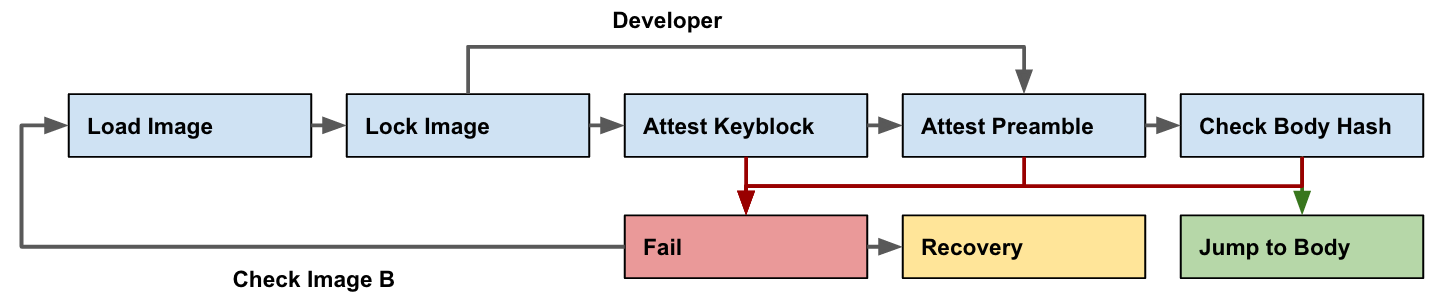
\includegraphics[width=0.8\linewidth]{lock_image.png}
  \caption[Verified Boot Program Flow w/ Locking]{The Vboot flow for locking the
      Image.
  }\label{fig:lock_flow}
\end{figure}

The flow in Image~\ref{fig:lock_flow} shows an example of how the hardware locking 
would be implemented.
This would prevent any Time of Check Time of Use (TOCTOU) Vulnerabilities that
would exist in the Verified Boot library.
A TOCTOU attack is when the attacker modifies data after it has been checked,
but before it is being used.
In Vboot's case a TOCTOU attack would modify the Image after it has been
attested, but before Vboot jumps to the start of the Image's code.

TOCTOU vulnerabilities are very common in secure programs\cite{tpm-toctou}.
Implementing memory locking would make it trivial to prove that the system has
no TOCTOU attack vectors. 
Until this feature is implemented, there will always be the possibility of a
TOCTOU attack.
This recommendation was brought to the attention of Google Engineer's through
the Chromium-OS email group.
Their response was that it is possible to implement under current hardware, and
it was recommended under NIST's ``Bios Protection Guidelines'', but it has not
been implemented yet.
There are examples of Secure Boot implementations that enable memory locking\cite{elane}.

% \section{Increased TPM Usage}
% 
% TODO: Do the hashing and encrypting on the TPM
% This would actually help because people could fake the hash
